\chapter{测试与评估}
\label{chap:evaluation}

在本章中,我们将对第四章介绍的AppShield系统进行测试与评估,这主要包括隐私问题检测与相似度检测部分。
在~\ref{sec:test-set}节中,我们简单介绍了经过两年时间收集的测试集;
在~\ref{sec:privacy-eval}节中我们对AppShield检测隐私问题的能力进行测试与评估,并挑选了被发现隐私问题样本数较高的广告库Tapjoy,进行了详细的案例分析;
在~\ref{sec:sim-eval}节中我们对AppShield使用的相似度检测方法进行了测试与评估。
最后在~\ref{sec:eval:conclusion}节中我们将对本章进行小结。

\section{测试集}
\label{sec:test-set}


AppShield系统的测试数据集主要来自于AppShield的爬虫程序,同时也包括一些已知的恶意软件库。
总计分析应用数量超过14万,应用文件数据量已经超过4.5TB磁盘空间,分析结果数据库约为45GB,表~\ref{tab:test-set}为测试集的基本情况。

\begin{table}
	\centering
	\bicaption[tab:test-set]{AppShield测试集}{AppShield测试集}{Table}{Test Set of AppShield}
	\begin{tabularx}{\textwidth}{|X|c|X|X|}
		\hline
		市场名字 & 应用数量 & 市场类型 & 链接\\
		\hline
		Google Play & 116672 & 北美、欧洲官方应用市场 & \url{https://play.google.com/store/apps}\\
		\hline
		Android Drawer & 6537 & 北美第三方市场 & \url{http://www.androiddrawer.com/}\\
		\hline
		酷安网 & 8171 & 国内第三方市场 & \url{http://www.coolapk.com/}\\
		\hline
		腾讯应用宝 & 10993 & 国内第三方市场 & \url{http://www.myapp.com/}\\
		\hline
		机锋网 & 1913 & 国内第三方市场 & \url{http://apk.gfan.com}\\
		\hline
		Android病毒基因库 & 1260 & 已知恶意应用库 & \url{http://www.malgenomeproject.org/}\\
		\hline
		美国North Eastern大学研究数据库 & 1278 + 3063 & 普通应用以及恶意样本 & 帮助美国科研团队评估科研成果有效性,\url{http://recon.meddle.mobi/}\\
		\hline
		用户上传 & 1366 & 任意 & 通过 \newline 
								\url{http://appaudit.io}\\
		\hline
	\end{tabularx}
\end{table}


我们的测试集具有以下特点:

\begin{enumerate}
	\item 涵盖官方与非官方的应用市场。
	\item 涵盖国内与国外的应用市场。
	\item 涵盖移动量的已知恶意应用,可以评估AppShield的有效性
\end{enumerate}

搜集的市场元数据包括:应用上传时间、大小、更新时间、Google Play评分、开发者名字、开发者联系方式、市场内相关应用、下载量、一些评论、分类tag、45款主流杀毒软件病毒检测结果、图标、展示图片、展示视频、内容分级、隐私报告等等。这些信息帮助我们对检测到的隐私问题的应用进行影响因子排序。

\section{隐私问题检测}
\label{sec:privacy-eval}

在AppShield中使用了AppAudit进行单应用审查。
其中AppAudit在基准病毒样本库Android Malware Genome Project上的测试准确度可以达到99.3\%,在检测时间上AppAudit可以在平均几秒钟的时间内完成一个应用的审查,并且审查一个应用的内存使用量只需要200MB以内,普遍优于现有学术研究以及Google应用市场的产品,对于AppAudit详细的测试评估可以参考AppAudit的论文。

对于应用市场内的隐私泄露情况,AppShield会总结出泄露应用列表以及泄露概要,来对市场内的隐私泄露情况进行评估与分析。

\subsection{隐私泄露情况总览}

在检测到的隐私泄露中,有些位于第三方库组件中,有些位于应用开发者自己开发的组件中。
我们将AppShield分析收集到的泄露信息进行汇总,并将属于应用本身的组件归纳为一类,记做“app\_itself”。
图~\ref{fig:leak-comp}为汇总之后,组件被检测出泄露信息频次最多的20个组件。

\begin{figure}
	\centering
	\includegraphics[width=1\textwidth]{figure/leak-comp.png}
	\bicaption[fig:leak-comp]{具有隐私问题的组件泄露情况}{具有隐私问题的组件泄露情况}{Fig}{Leakage Information of Problematic Components}
\end{figure}

从图中可以看出,应用本身的隐私泄露情况是最普遍的,大约占据3成左右,剩下的7成都是第三方组件库导致的隐私泄露问题。
前20个隐私泄露频次最多的组件中,第三方广告库就占有着很大的比例,其中Tapjoy、Mobfox都是流行度比较高的广告库,在Appbrain对官方Google Play市场的份额统计中,已安装应用分别有5.66\%、0.73\%的应用使用了这两家广告库(达到5.66万个以及7300个应用使用这些有问题的库)。
由于广告库是这次分析隐私泄露的重灾区,我们会在之后的问题部件案例分析中着重介绍。

\begin{figure}
	\centering
	\includegraphics[width=0.7\textwidth]{figure/leak-type.png}
	\bicaption[fig:leak-type]{泄露隐私数据类型分布}{泄露隐私数据类型分布}{Fig}{Distribution of Leakage Information Type}
\end{figure}

我们以泄露的信息为关注点,图~\ref{fig:leak-type}为在所有组件中泄露隐私信息类型的情况分布图。

可以看出泄露情况最严重的是IMEI,即国际移动设备标识,占总泄露频次的83.5\%。
IMEI是手机的唯一识别号码,由15位数字组成,前6位数是“型号核准号码”(TAC,Type Approval Code),代表机型。接着的2位数为“最后装配号”(FAC,Final Assembly Code),代表产地。之后的6位数是“串号”(SNR,Serial Number),代表生产顺序号。最后1位数通常是“0”,为检验码。

IMEI本身包含的隐私信息有限,但是IMEI经常被应用用来当作识别一个手机的标识。
所以如果IMEI被泄露,可能会存在潜在的安全隐患。
WhatsApp在三年前被曝光使用手机的号码当作用户名,使用IMEI的md5值作为密码。
在这种情况下,IMEI被泄露就相当于WhatsApp的密码被泄露,是一个严重的安全隐患。

除开IMEI之外,其他的隐私信息的泄露情况也是不可忽视的。
相比IMEI,电话号码以及地理位置相关的隐私信息被泄露带来的安全隐患可能大得多,所以应用的隐私泄露是一个需要被应用市场关注的领域。

\subsection{问题组件分析}

针对泄露隐私问题最严重的广告类库,我们挑选了检测出泄露情况较多的几个广告库进行了作为样例进行数据汇总以及可视化。
根据AppShield的问题组件分析,找出对应广告库的不同版本,并获取应用不同版本广告库的引用的单应用审查结果,最终得出统计结果。
并且,我们着重对Tapjoy进行了详细的案例分析。

\begin{table}
	\centering
	\bicaption[tab:adlib-overview]{广告库相关基本信息}{广告库相关基本信息}{Table}{General Information of Related Advertise Libraries}
	\begin{tabularx}{\textwidth}{|c|c|c|X|}
		\hline
		广告库 & 地区 & 成立时间 & 特点\\
		\hline
		Tapjoy & 北美 & 2007 & 活跃用户高 覆盖面广\\
		\hline
		Mdotm & 北美 & 2009 & 基于表现的广告投放 跨渠道\\
		\hline
		MobFox & 欧洲 & 2010 & 针对欧洲 提供广告服务端和应用优化服务\\
		\hline
	\end{tabularx}
\end{table}

\begin{table}
	\centering
	\bicaption[tab:adlib-leak]{广告库在AppShield中的分析结果统计数据}{广告库在AppShield中的分析结果统计数据}{Table}{Analysis Statistics of AppShield for Advertise Library}
	\begin{tabular}{|c|c|c|c|c|}
		\hline
		广告库 & 泄露样本数 & 总样本数 & 泄露版本数 & 总版本数\\
		\hline
		Tapjoy & 379 & 3447 & 31 & 103\\
		\hline
		Mdotm & 77 & 92 & 2 & 2\\
		\hline
		MobFox & 163 & 178 & 12 & 12\\
		\hline
	\end{tabular}
\end{table}


我们一共挑选了三个广告库样例,分别为Tapjoy,MdotM(已更名为CrossChannel)以及MobFox。
表~\ref{tab:adlib-overview}介绍了三个广告库的基本信息以及特点。

在AppShield深度问题组件分析中,Tapjoy组件被识别一共有103个版本,其中31个版本被AppAudit检测出有隐私泄露行为;
MobFox的版本总量相对Tapjoy少了很多,仅有12个版本,并且12个版本均被AppShield检测出有隐私泄露行为;
而MdotM(CrossChannel)仅被检测出在测试集中有2个样本,并且2个样本均有泄露隐私行为。
图~\ref{fig:leak}为不同广告库版本在测试集中的使用情况,其中红色的表明被检测出隐私泄露的数量。
表~\ref{tab:adlib-leak}为这三个广告库在AppShield中检测的相关数据。

\begin{figure}
  \centering
  \subfigure[Tapjoy]{
    \label{fig:leak:tapjoy} %% label for first subfigure
    \includegraphics[width=1\textwidth]{figure/tapjoy-leak.png}
  }

  \subfigure[MobFox]{
    \label{fig:leak:mobfox} %% label for second subfigure
    \includegraphics[width=0.4\textwidth]{figure/mobfox-leak.png}
  }
  \subfigure[Mdotm]{
  	\label{fig:leak:mdotm}
  	\includegraphics[width=0.4\textwidth]{figure/mdotm-leak.png}
  }
  \bicaption[fig:leak]{不同版本广告库泄露隐私情况}{不同版本广告库泄露隐私情况}{Fig}{Sensitive Information Leak among Different Versions of Ad Lib SDK}
\end{figure}

Tapjoy是一家美国的移动广告平台,成立于2007年,目前覆盖了10亿台全球移动设备,全球月活跃用户高达5.05亿。
应用开发者能利用Tapjoy的SDK,在应用中插入Tapjoy提供的广告,因而来将应用的流量变现。

在AppShield的分析中检测出Tapjoy组件会在应用运行的过程中会泄露手机的IMEI信息,我们接着对出现问题的应用进行反编译,确认了泄露的路径,并整理出了Tapjoy在工作过程中会收集并且通过HTTP传输出去的信息。
表~\ref{tab:tapjoy-leak}为我们分析得出的Tapjoy SDK会收集的用户信息列表,我们对敏感数据进行了标红处理。

\begin{table}
	\centering
	\bicaption[tab:tapjoy-leak]{Tapjoy SDK收集的用户信息}{Tapjoy SDK收集的用户信息}{Table}{User Information List of Tapjoy SDK will Collect}
	\begin{tabularx}{\textwidth}{|l|X|}
		\hline
		参数名 & 描述\\
		\hline
		app\_id & Tapjoy开发者对应的app\_id\\
		\hline
		android\_id & 用户第一次打开设备时随机生成的一个64位的数字字符串,当用户恢复出厂设置时,这个值会重新随机生成\\
		\hline
		{\color{red}udid} & IMEI\\
		\hline
		sha2\_udid & IMEI的SHA-256\\
		\hline
		sha1\_mac\_address & 设备mac地址的SHA-1\\
		\hline
		serial & 硬件的串号\\
		\hline
		device\_name & 终端用户的设备名称\\
		\hline
		device\_manufacturer & 设备的制造商\\
		\hline
		os\_version & 操作系统版本\\
		\hline
		country\_code & 国家代码\\
		\hline
		language\_code & 语言代码\\
		\hline
		{\color{red}package\_names} & 设备当前安装的应用列表\\
		\hline
	\end{tabularx}
\end{table}


之前讨论了泄露IMEI的危害,在Tapjoy SDK中,还会尝试去获得设备当前安装的应用列表,这其实也是一个比较敏感的信息。
之前有案例是通过手机病毒获取受害者手机上安装的应用列表,从而得知用户手机中是否安装了银行类的应用,利用这个信息使用社会工程学进行诈骗。

\begin{figure}
	\centering
	\includegraphics[width=0.6\textwidth]{figure/privacy-policy.png}
	\bicaption[fig:privacy-policy]{Tapjoy官方网站隐私声明}{Tapjoy官方网站隐私声明}{Fig}{Privacy Policy of Tapjoy}
\end{figure}

图~\ref{fig:privacy-policy}展示了Tapjoy在官网中声明的Tapjoy SDK会收集的信息。
Tapjoy声称会将手机到的用户信息安全保护好,不允许未授权机构或个人访问。
另外Tapjoy会将用户信息与合作伙伴、Tapjoy相关分支机构以及广告商等共享,从而给用户提供更好的广告服务。

从图~\ref{fig:leak:tapjoy}可以看出,Tapjoy SDK更新比较活跃,有隐私泄露行为的版本只占了总版本数的一小部分。
并且在最新的SDK版本中(v10.2.2),Tapjoy也添加了将IMEI进行SHA-256的代码,只使用IMEI哈希之后的值。
这样就能将隐私信息进行匿名化,同时能同样标识用户的设备。
图~\ref{fig:tapjoy-code}为Tapjoy SDK对IMEI进行SHA-256匿名化的代码片段。

\begin{figure}[!h]
	\centering
	\begin{lstlisting}[language={java}]
	if (isPermissionGranted("android.permission.READ_PHONE_STATE")) {
		try {
			if (getConnectFlagValue(TapjoyConnectFlag.DEBUG_DEVICE_ID) == null || getConnectFlagValue(TapjoyConnectFlag.DEBUG_DEVICE_ID).length() <= 0) {
				deviceID = telephonyManager.getDeviceId();
			} else {
				deviceiD = getConnectFlagValue(TapjoyConnectFlag.DEBUG_DEVICE_ID);
			}
			TapjoyLog.i(TAG, "deviceID: " + deviceID);
			...
			if (validDeviceID) {
				sha2DeviceID = TapjoyUtil.SHA256(deviceID);
				return;
			}
			...
		}
	}
	\end{lstlisting}
	\bicaption[fig:tapjoy-code]{最新版本Tapjoy SDK中对IMEI进行了SHA-256操作的相关代码}{最新版本Tapjoy SDK v10.2.2中对IMEI进行了SHA-256操作的相关代码}{Fig}{Code Snippet of Tapjoy SDK v10.2.2}
\end{figure}



另外在进行案例分析中,我们发现MobFox和Mdotm组件的所有版本都有被检测出泄露隐私信息行为的样本,但是仍有一小部分同版本的样本没有被AppAudit检测出有安全隐患。

从图~\ref{fig:leak:mobfox}中可以看到,MobFox第二条直方一共存在130多个应用使用了同一个Mobfox SDK版本。
然而在这130多个应用中有将近120个被AppAudit识别出存在隐私问题,由此可以推断未被标记的10多个应用很可能就是AppAudit存在遗漏的有隐私问题的样本。
这些样本可以帮助AppAudit开发者快速找到遗漏样本并对工具本身进行修正。
同样的如果途中某个版本大量样本没有问题,只有少数被标记,则可以推断这些被标记的样本可能是单应用审查工具的误报案例,同样可以帮助这类工具。
在AppShield中由于AppAudit设计中不会出现误报,只有遗漏,所以相应的在AppShield的分析中只会出现某个版本的样本中疑似有遗漏。

\section{相似度检测}
\label{sec:sim-eval}

我们还对提出的相似度检测的方法进行了测试评估。
我们首先对相似度检测方法处理混淆能力、检测时间进行了测试。
之后我们挑选了10种第三方库以及他们的不同版本,一共53个SDK,来对我们测试集中10993个来自腾讯应用宝市场上的应用进行了第三方库检测,来检验我们的相似度检测方法是否在给出问题组件的前提下,找出包含问题组件的应用。
最后我们还挑选了1000个应用,对其进行了重打包应用的检测。

\subsection{微基准测试}

在微基准测试中,我们人工编写了集成了多个第三方库的应用,并使用此应用的未混淆版本以及经过了不同配置后的混淆处理之后的应用进行相似度检测,从而检验本文的相似度检测方法是否有能力处理混淆。

我们编写的应用一共集成了4个第三方库,处理JSON的工具库gson,提供类型安全的HTTP客户端retrofit,另外还有retrofit依赖的两个库okhttp和okio。

由于代码缩减的检测依赖于应用对第三方库的使用情况,所以我们在应用中对几个第三方库进行了基本功能的使用,从而模拟真实应用的情况。我们的对照组为未混淆过的应用,实验组有6个。

\begin{table}
	\centering
	\bicaption[tab:micro-bench]{相似度检测微基准测试结果}{相似度检测微基准测试结果}{Table}{Micro-benchmark Result of Similarity Detection}
	\begin{tabular}{|c|c|c|c|c|c|c|}
		\hline
		 & 标识符重命名 & 平铺化包 & 重打包类 & 代码缩减 & 代码优化 & 相似度\\
		\hline
		试验组1 & 1 & 0 & 0 & 0 & 0 & 1\\
		\hline
		试验组2 & 0 & 1 & 0 & 0 & 0 & 1\\
		\hline
		试验组3 & 0 & 0 & 1 & 0 & 0 & 0.21\\
		\hline
		试验组4 & 0 & 0 & 0 & 1 & 0 & 0.63\\
		\hline
		试验组5 & 0 & 0 & 0 & 0 & 1 & 0.8\\
		\hline
		试验组6 & 1 & 1 & 0 & 1 & 0 & 0.75\\
		\hline
	\end{tabular}
\end{table}


实验结果如表~\ref{tab:micro-bench}所示,可以看出我们的相似度检测方法可以很好的应对标识符重命名、代码缩减以及代码优化,能在一定程度上处理包平铺化,对重打包类处理能力较差。
主要是因为我们利用了包的层次信息,包平铺化只会在一定程度上保留包层次信息,而重打包类完全破坏了此信息。

但是在实验中我们也发现了重打包类混淆技术的一些特点。
由于重打包类会将所有混淆的类重新打包到一个新的包中,所以当我们发现一个包中的类匹配了来自很多不同包内的类时,可能此包为重打包混淆中的新包。
以此发现为基准,可能可以发明一些启发式的算法,来发现应用是否经过了重打包混淆,并尝试进行识别。

在指纹生成阶段,一共包括4个步骤:
\begin{enumerate}
	\item 解压缩apk包
	\item 使用baksmali将dex代码反编译成smali代码
	\item 解析smali代码,将其结构化以便生成指纹
	\item 对稳定特性进行SHA1指纹生成
\end{enumerate}

图~\ref{fig:fingerprint-time}展示了10993个应用在指纹生成过程中每一步所花费的时间,可以看出SHA1生成指纹这一步明显随着类的数量增加而提升,而其余几步随着类的增加基本趋于稳定。

\begin{figure}
	\centering
	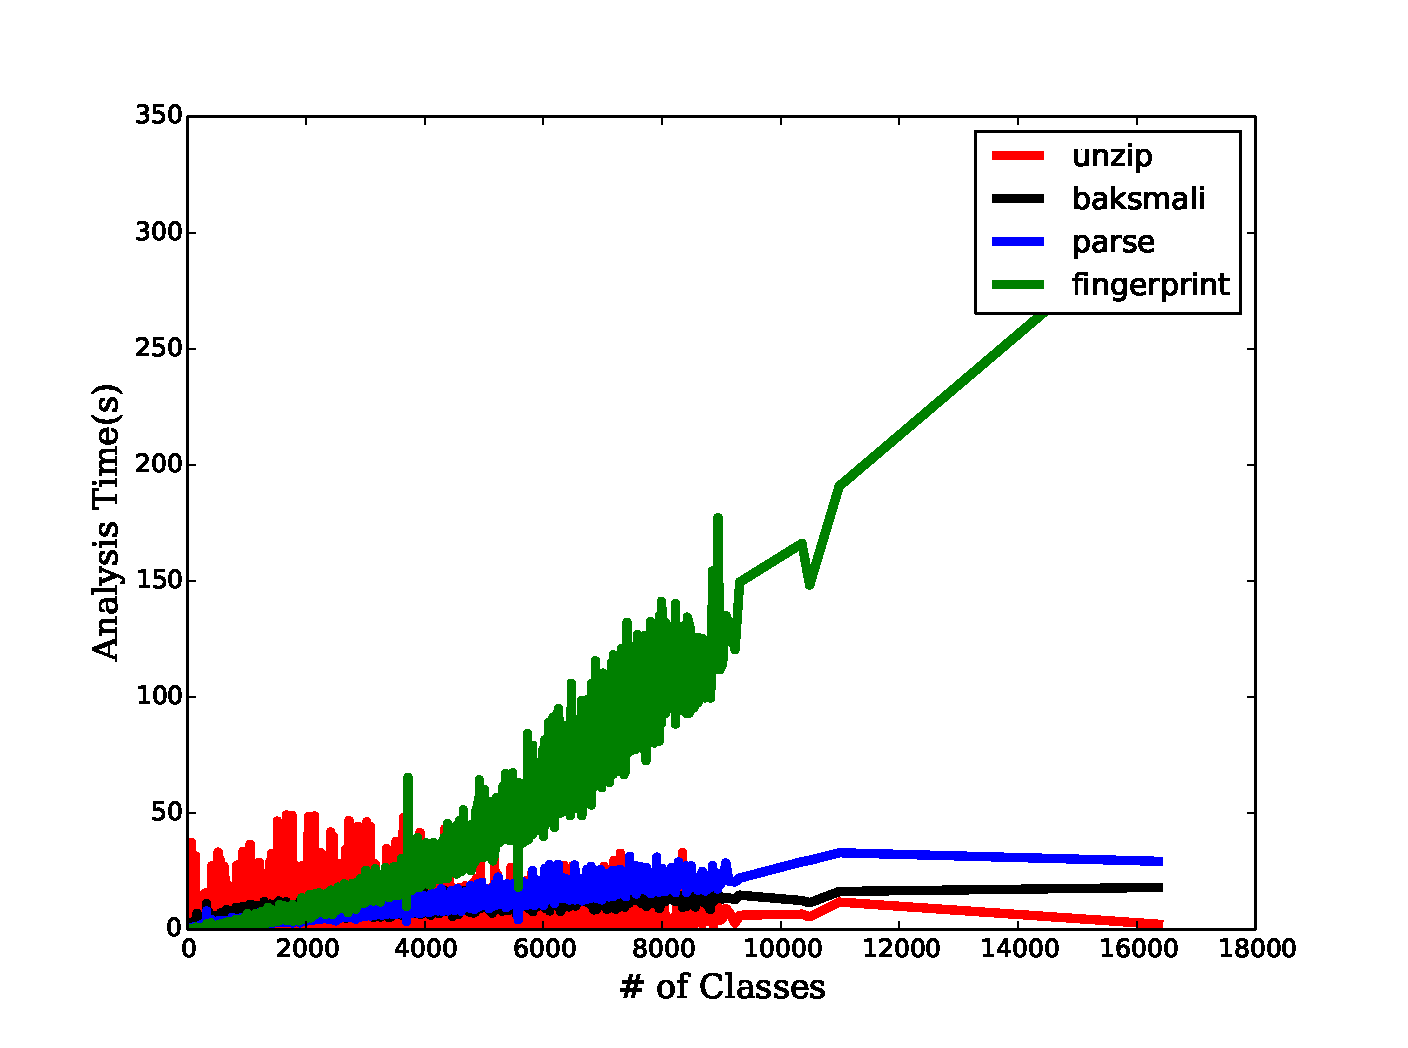
\includegraphics[width=0.8\textwidth]{figure/time-cdf.eps}
	\bicaption[fig:fingerprint-time]{指纹生成各部分时间CDF图}{指纹生成各部分时间CDF图}{Fig}{CDF of Different Part of Time in Fingerprint Generate}
\end{figure}

\subsection{第三方库检测}

在第三方库检测的实验中,我们人工获取了6个第三方库的67个SDK版本。
表~\ref{tab:sdk-overview}为这些SDK的基本信息。

\begin{table}
	\centering
	\bicaption[tab:sdk-overview]{SDK相关信息}{SDK相关信息}{Table}{Information of Selected SDK}
	\begin{tabularx}{\textwidth}{|X|X|X|c|}
		\hline
		SDK名 & 包名 & 功能 & 版本数\\
		\hline
		gson & \texttt{com.google.gson} & 提供JSON相关操作 & 20\\
		\hline
		okhttp & \texttt{com.squareup.okhttp3} & HTTP客户端 & 12\\
		\hline
		retrofit & \texttt{com.squareup.retrofit}\newline\texttt{com.squareup.retrofit2} & 类型安全的HTTP客户端 & 15\\
		\hline
		weibo核心SDK & \texttt{com.sina.weibo}\newline\texttt{com.sina.sso} & 提供微博接入相关功能 & 6\\
		\hline
		友盟SDK & \texttt{com.umeng.analytics} & 提供应用统计相关功能 & 13\\
		\hline
		Talking Data SDK & \texttt{com.tendcloud.tenddata} & 提供应用统计相关功能 & 1\\
		\hline
	\end{tabularx}
\end{table}

10993个应用的检测结果如表~\ref{tab:third-detect}所示,在使用的这来自6个第三方库的67个SDK版本检测中,至少被检测出含有一个第三方库的应用有1803个,占全部的16.4\%。
其中gson检测率最高,被1230个应用使用,占全部的10.26\%。

\begin{table}
	\centering
	\bicaption[tab:third-detect]{第三方库检测结果}{第三方库检测结果}{Table}{Analysis Result of Third-Party Library Detection}
	\begin{tabular}{|c|c|c|}
		\hline
		SDK & 应用数 & 比例\\
		\hline
		gson & 1230 & 10.26\%\\
		\hline
		友盟SDK & 748 & 6.24\$\\
		\hline
		Weibo核心SDK & 282 & 2.35\%\\
		\hline
		okhttp & 85 & 0.71\%\\
		\hline
		retrofit & 58 & 0.48\%\\
		\hline
		Talking Data SDK & 15 & 0.13\%\\
		\hline
	\end{tabular}
\end{table}


本实验为原型实验,证明了第三方库检测的可行性。
之后可以通过持续从maven数据库获取第三方库的SDK来建立完备的第三方库数据库,对应用实现更全面准确的检测。

\subsection{克隆应用检测}

在检测结果中有很多只含有一个包的应用,并且这些应用之间的相似度都为1。
我们人工分析了这些“特殊”的应用,发现这些应用是通过了奇虎360加固保处理后的应用,这些应用一共有1270个。
360加固保使用通常我们说的应用“加壳”的方式对应用进行保护,通过重打包,对应用代码进行加密、运行时完整性检验等方式防止应用被篡改以及被分析。
我们将结果中所有使用了奇虎360加固保处理的应用结果剔除,来防止其对测试集造成的影响。

我们一共挑选了1000个应用进行克隆应用的检测,一共存在499500个比对结果。
图~\ref{fig:sim-cdf}为应用相似度的CDF图。

\begin{figure}
	\centering
	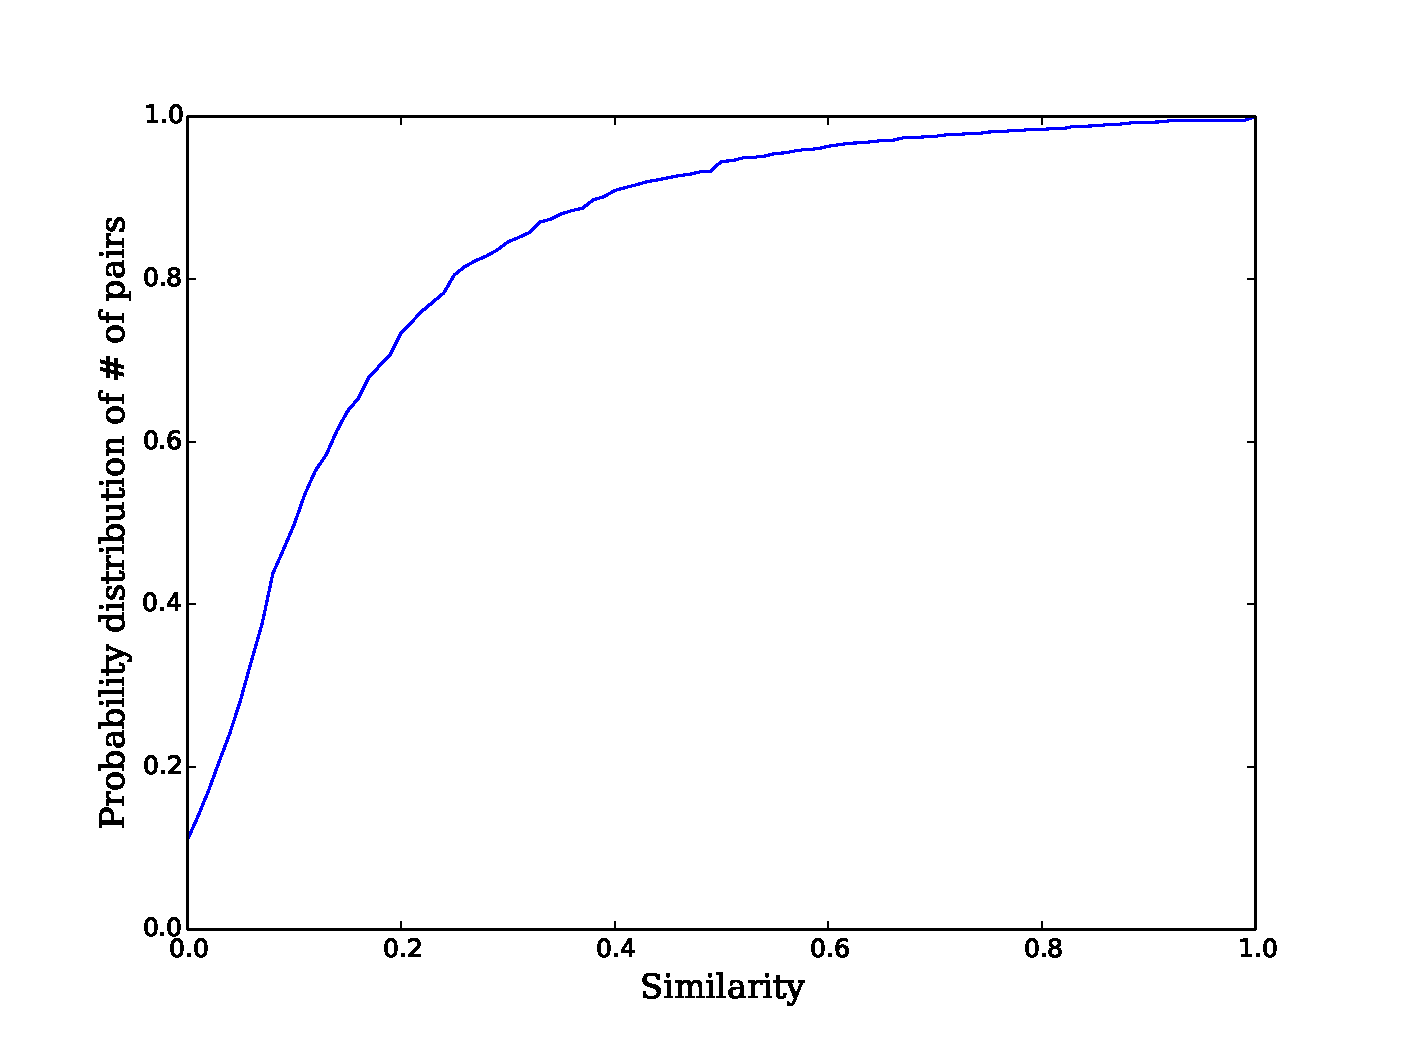
\includegraphics[width=0.6\textwidth]{figure/sim-cdf.eps}
	\bicaption[fig:sim-cdf]{应用相似度CDF图}{应用相似度CDF图}{Fig}{CDF of Similarity between Applications}
\end{figure}

从图中可知,高于在克隆应用检测阶段设置的相似度阈值0.9的有0.7\%的应用。

在我们检测出的潜在克隆应用对中,我们人工确认了一例开发者以不同应用名将同一应用上传应用市场多次的事例。
图~\ref{fig:clone-app}为这一对应用,这一对应用的相似度为1,开发者密钥相同,但有着不同的包名以及应用名。
这说明着,在中国市场上的确存在开发者仅修改应用名和包名,就将同一应用多次上传至应用市场,来提高应用的曝光的可能性。

\begin{figure}
	\centering
	\includegraphics[width=0.6\textwidth]{figure/clone-pair.png}
	\bicaption[fig:clone-app]{不同应用名的相同应用}{不同应用名的相同应用}{Fig}{Same Application of Different Application Names in Myapp}
\end{figure}

可以看出,我们的克隆应用检测误报率很高。
在经过对误报样本进行人工确认之后发现,很多相似度很高的应用只是因为使用了相同的第三方库,而应用本身逻辑在应用所有代码中占比很小。
所以如果需要提高检测的准确性,需要剔除掉应用使用的第三方库,找出应用真正的逻辑,进行比对。

\section{本章小结}
\label{sec:eval:conclusion}

在本章中,我们对AppShield的隐私问题分析以及相似度检测两方面进行了测试与评估。
测试集一共包含13万多的应用,来自国内外各大应用市场。
首先我们对AppShield的隐私问题分析部分进行了测试。
在测试集中,我们成功分析了14万样本,找到超过9000多例的隐私泄露应用,并总结出超过20个有隐私问题的问题部件,并对隐私泄露方式进行了总结与可视化。
然后我们对AppShield的相似度检测部分进行了测试评估。
我们选取了来自腾讯应用宝市场的10993个应用进行了第三方库的检测,对8个第三方库的67个SDK版本进行检测,最终检测出超过10\%的应用包含gson库,超过6\%的应用包含友盟SDK。
结果验证了相似度检测的方法能够较好的应用与第三方库的检测中。
最后我们挑选了1000个应用进行克隆应用检测,最终检测出一例开发者以不同应用名将应用重复上传至应用市场的事例。